\section{Contact-graph study sensitivity evidence}\label{sec:historical-evidence}
\subsection{Coverage, provenance and statistical units}
Table~\ref{tab:hist-coverage} separates the evidence layers and the five batches
within the contact-graph study extension. Contact graphs retain the first 65\% of complete
timestamp groups. Undirected contacts become reciprocal propagation arcs;
repeated events are collapsed for topology and counted for event-weighted
degree. Propagation probability remains uniform, independently of these counts.
The initial study's protocol and 42 configuration records establish its coverage;
its outputs are not pooled with the later extension or the SNAP study.
\begin{longtable}{p{.23\linewidth}p{.51\linewidth}p{.14\linewidth}}
\caption{Evidence layers and experiment coverage. A configuration fixes graph, replicate, $k,p,h,W$ and coupling; a method changes eligibility. Replicates are repeated seed-selection runs. Counts are not independent network sample sizes.}\label{tab:hist-coverage}\\
\toprule Batch / graphs & Selection design and evaluation & Configs. / runs\\\midrule\endfirsthead
\multicolumn{3}{l}{\tablename~\thetable{} (continued)}\\\toprule
Batch / graphs & Selection design and evaluation & Configs. / runs\\\midrule\endhead\bottomrule\endfoot
Initial study / C4, C3 & C4: $k=5$; C3: $k=20$. $p=.01$, $h=3$, $W=20,80,320$, step; two replicates (301--302); $M=2000$. Initial weighted-pool/reference comparisons. & 42 / 168\\
Contact-graph study budget / C4 & $k=5$, $p=.01$, $h=3$, $W=20,80,320,1280,5120$, step; ten replicates (1001--1010); $M=10{,}000$. Reference-budget sensitivity. & 200 / 1800\\
Contact-graph study parameters / C4 & $k=5$, $W=320$, step; $(p,h)=(.005,3),(.05,3),(.01,1),(.01,5)$; ten replicates; $M=10{,}000$. Local parameter changes. Default $(.01,3)$ reuses 40 budget configurations. & 160 / 1440\\
Contact-graph study coupling / C4 & $k=5$, $p=.01$, $h=3$, $W=320,1280$, fixed edge; ten replicates; $M=10{,}000$. Coupling-specific comparisons and budget transitions. & 80 / 720\\
Contact-graph study larger seeds / C3 & $k=20$, $p=.01$, $h=3$, $W=320,1280$, step; ten replicates; $M=10{,}000$. Seed-budget and coverage control. & 60 / 540\\
Synthetic controls / S2 & $k=5$, $p=.01$, $h=3$, $W=80,320$, step; five replicates (1001--1005) per fixed instance; $M=10{,}000$. Topology controls. & 20 / 180\\
SNAP primary / E3 & $k=5$, $p=.01$, $h=3$, $W=80,320,1280$, step; five replicates (1101--1105); $M=10{,}000$. SNAP transfer, budget and pool coverage. & 45 / 390\\
SNAP coupling / E3 & $k=5$, $p=.01$, $h=3$, $W=320$, fixed edge; three replicates (1101--1103); $M=10{,}000$. Coupling control. & 9 / 78\\
Post-hoc precision / E3 & PageRank-4k/5\% at the tighter tolerance, $W=80,320,1280$, step; other settings, five replicates and $M=10{,}000$ reused from primary study. Existing full references reused. Numerical sensitivity, not new independent replication. & 45 / 90\\
\end{longtable}
\noindent C4: invs2013 ($n=91$), invs2015 (212), kenya2012 (75), sfhh2009 (402).
C3 excludes sfhh2009. S2: one BA and one SBM instance, each $n=2000$.
E3: CollegeMsg (1438), ca-GrQc (5241), wiki-Vote (7115).
Contact-graph study extension totals are $200+160+80+60+20=520$ configurations and 4680 methods.
Its nine methods are full selection, Weighted-2k/4k/8k, Degree-4k, PageRank-4k and three random-4k pools.
The SNAP matrix totals 54 configurations and 468 methods. Resource-only preflight is outside all outcome totals.


The 520-configuration extension specified its protocol after the initial study
and resource preflight. It is not a public preregistration. All nine methods use
the complete propagation graph and differ only in seed eligibility, with a
common lexical tie rule. Candidate sizes are capped at the number of vertices.
The namespace is \texttt{computing-extension-20261015-v1}; selection and evaluation
families have separate hash keys. Selection budgets use nested world prefixes for every method. At each $W$, both full and restricted methods select seeds anew; the 10,000-world evaluation family stays fixed across budgets within each graph/replicate/coupling.
PageRank in the contact-graph study uses the pre-specified default numerical settings; these controls
are distinct from the SNAP post-hoc tolerance study.

The contact-graph study summary audit covers all 520 stored JSON/NPZ pairs. Their 1,040 file
hashes match the result manifest, and the contact-graph study engine hash matches the
SNAP package's legacy engine. Means, paired differences and conditional
Monte Carlo standard errors are recomputed from all 4,680 saved method vectors,
each containing 10,000 counts. Seven replicate-level method summaries result after
averaging the three random pools within each replicate. The 3,640 replicate rows,
378 group rows (reported means and sample standard deviations) and 240 adjacent
budget transitions agree with the saved analyses. This verifies file integrity
and the specified numerical summaries, not every aspect of the study design.
These checks reaggregate saved results; they do not replay selection or propagation.

For each replicate, $\Delta$ is restricted minus full mean spread. The reported loss
is $-100\Delta/(\widehat\sigma_{\rm full}-k)$, averaged across replicates after forming
each replicate's ratio; all denominators are positive. A negative loss denotes a
point-estimate gain. Table SDs describe variation across replicates, not confidence
intervals for a population of networks. Conditional Monte Carlo standard errors
come from the paired per-world differences for fixed selected sets. Random-pool
vectors are averaged before calculating their conditional errors; the pools do
not triple the replicate count. The same replicate used at multiple settings is a repeated
measurement. No new hypothesis tests are introduced here, and no contact-graph study
replicates are pooled with the five SNAP replicates.

\subsection{Local propagation-parameter changes}
Table~\ref{tab:hist-parameters} and Fig.~\ref{fig:hist-parameters} include all
four preselected nondefault settings and the reused default setting at $W=320$.
They vary probability or horizon around the default, rather than forming a full
factorial design. Over the 160 nondefault configurations, Degree-4k and PageRank-4k
reproduce 117 and 132 ordered full-reference trajectories. Each has one negative
paired spread difference; positive differences occur in 42 and 27 configurations,
respectively. Weighted-4k reproduces none of these trajectories and has 117
negative and 43 positive differences. These counts summarize the retained
configurations; they are not independent Bernoulli trials.

The weighted-ranking discrepancy varies with graph and setting. At $(p,h)=(.05,3)$,
its mean differences are $-0.51309$, $-1.52602$, $+0.07939$ and $-4.98321$ nodes
for invs2013, invs2015, kenya2012 and sfhh2009, respectively. The corresponding
mean incremental losses are 4.12\%, 2.37\%, $-0.89$\% and 4.09\%.
Thus neither a single sign nor the absolute difference alone summarizes the
parameter control. Complete results for Weighted-2k/8k and the within-replicate
random mean remain in the accompanying all-method CSVs.
\begin{figure}[p]
\centering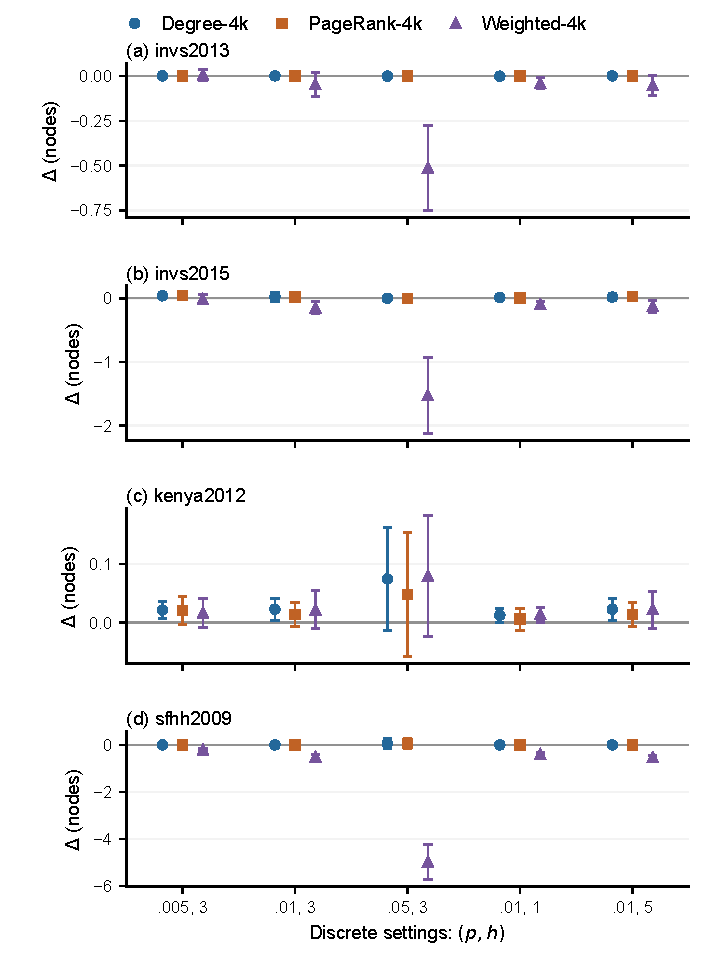
\includegraphics[width=\linewidth]{HistoryParameters.pdf}
\caption{Contact-graph study parameter sensitivity for three 4k rankings, with $k=5$,
$W=320$ and step coupling. Each panel is one contact graph; each point is the mean
paired spread difference over ten replicates, and bars are one replicate standard deviation.
Settings are discrete, not a continuous sweep. Vertical scales differ between
panels. Positive differences favor the restricted set. The default $(.01,3)$
reuses the budget scan. These are replicate-variation bars, not conditional Monte Carlo
intervals or uncertainty across networks.}\label{fig:hist-parameters}
\end{figure}
\FloatBarrier
\begin{longtable}{llrrrrr}
\caption{Contact-graph study propagation-parameter sensitivity at $k=5$, $W=320$, step coupling. D, P and W denote Degree-4k, PageRank-4k and Weighted-4k. $\Delta$ is restricted minus full spread (nodes); SD is across replicates; loss is the mean pathwise incremental loss (\%), negative when restricted spread exceeds full-reference spread. Match counts refer to the entire ordered sequence. Coverage is the fraction of eligible vertices (\%). The default $(.01,3)$ rows reuse the budget scan; they are not additional configurations.}\label{tab:hist-parameters}\\
\toprule
$(p,h)$ & Rank & $\overline\Delta$ & SD & Loss & Match & Cov. \\
\midrule
\endfirsthead
\multicolumn{7}{l}{\tablename~\thetable{} (continued)}\\
\toprule
$(p,h)$ & Rank & $\overline\Delta$ & SD & Loss & Match & Cov. \\
\midrule
\endhead
\bottomrule
\endfoot
\multicolumn{7}{l}{\textit{invs2013}}\\*
0.005, 3 & D & +0.0016 & 0.0068 & -0.25 & 8/10 & 21.98\\*
0.005, 3 & P & +0.0016 & 0.0068 & -0.25 & 8/10 & 21.98\\*
0.005, 3 & W & +0.0044 & 0.0301 & -0.76 & 0/10 & 21.98\\*
0.01, 1 & D & +0.0000 & 0.0000 & +0.00 & 10/10 & 21.98\\*
0.01, 1 & P & +0.0000 & 0.0000 & +0.00 & 10/10 & 21.98\\*
0.01, 1 & W & -0.0386 & 0.0309 & +2.85 & 0/10 & 21.98\\*
0.01, 3 & D & +0.0014 & 0.0046 & -0.10 & 9/10 & 21.98\\*
0.01, 3 & P & +0.0014 & 0.0046 & -0.10 & 9/10 & 21.98\\*
0.01, 3 & W & -0.0467 & 0.0664 & +2.93 & 0/10 & 21.98\\*
0.01, 5 & D & +0.0014 & 0.0045 & -0.09 & 9/10 & 21.98\\*
0.01, 5 & P & +0.0014 & 0.0045 & -0.09 & 9/10 & 21.98\\*
0.01, 5 & W & -0.0507 & 0.0553 & +3.22 & 0/10 & 21.98\\*
0.05, 3 & D & +0.0000 & 0.0000 & +0.00 & 10/10 & 21.98\\*
0.05, 3 & P & +0.0000 & 0.0000 & +0.00 & 10/10 & 21.98\\*
0.05, 3 & W & -0.5131 & 0.2380 & +4.12 & 0/10 & 21.98\\
\multicolumn{7}{l}{\textit{invs2015}}\\*
0.005, 3 & D & +0.0385 & 0.0413 & -2.25 & 5/10 & 9.43\\*
0.005, 3 & P & +0.0392 & 0.0459 & -2.31 & 5/10 & 9.43\\*
0.005, 3 & W & -0.0186 & 0.0709 & +0.93 & 0/10 & 9.43\\*
0.01, 1 & D & +0.0124 & 0.0391 & -0.43 & 9/10 & 9.43\\*
0.01, 1 & P & +0.0063 & 0.0198 & -0.21 & 9/10 & 9.43\\*
0.01, 1 & W & -0.0986 & 0.0486 & +3.23 & 0/10 & 9.43\\*
0.01, 3 & D & +0.0200 & 0.0632 & -0.47 & 9/10 & 9.43\\*
0.01, 3 & P & +0.0200 & 0.0632 & -0.47 & 9/10 & 9.43\\*
0.01, 3 & W & -0.1500 & 0.0940 & +3.35 & 0/10 & 9.43\\*
0.01, 5 & D & +0.0186 & 0.0588 & -0.42 & 9/10 & 9.43\\*
0.01, 5 & P & +0.0242 & 0.0515 & -0.53 & 8/10 & 9.43\\*
0.01, 5 & W & -0.1327 & 0.0929 & +2.89 & 0/10 & 9.43\\*
0.05, 3 & D & +0.0000 & 0.0000 & +0.00 & 10/10 & 9.43\\*
0.05, 3 & P & +0.0000 & 0.0000 & +0.00 & 10/10 & 9.43\\*
0.05, 3 & W & -1.5260 & 0.5980 & +2.37 & 0/10 & 9.43\\
\multicolumn{7}{l}{\textit{kenya2012}}\\*
0.005, 3 & D & +0.0214 & 0.0142 & -4.45 & 0/10 & 26.67\\*
0.005, 3 & P & +0.0210 & 0.0238 & -4.43 & 3/10 & 26.67\\*
0.005, 3 & W & +0.0165 & 0.0246 & -3.47 & 0/10 & 26.67\\*
0.01, 1 & D & +0.0125 & 0.0117 & -1.33 & 4/10 & 26.67\\*
0.01, 1 & P & +0.0059 & 0.0188 & -0.67 & 9/10 & 26.67\\*
0.01, 1 & W & +0.0138 & 0.0127 & -1.47 & 0/10 & 26.67\\*
0.01, 3 & D & +0.0228 & 0.0185 & -2.10 & 3/10 & 26.67\\*
0.01, 3 & P & +0.0135 & 0.0205 & -1.24 & 6/10 & 26.67\\*
0.01, 3 & W & +0.0218 & 0.0323 & -2.01 & 0/10 & 26.67\\*
0.01, 5 & D & +0.0228 & 0.0184 & -2.09 & 3/10 & 26.67\\*
0.01, 5 & P & +0.0136 & 0.0207 & -1.25 & 6/10 & 26.67\\*
0.01, 5 & W & +0.0220 & 0.0317 & -2.03 & 0/10 & 26.67\\*
0.05, 3 & D & +0.0745 & 0.0878 & -0.83 & 1/10 & 26.67\\*
0.05, 3 & P & +0.0481 & 0.1057 & -0.54 & 7/10 & 26.67\\*
0.05, 3 & W & +0.0794 & 0.1031 & -0.89 & 0/10 & 26.67\\
\multicolumn{7}{l}{\textit{sfhh2009}}\\*
0.005, 3 & D & +0.0000 & 0.0000 & +0.00 & 10/10 & 4.98\\*
0.005, 3 & P & +0.0041 & 0.0130 & -0.12 & 9/10 & 4.98\\*
0.005, 3 & W & -0.2285 & 0.0591 & +6.32 & 0/10 & 4.98\\*
0.01, 1 & D & +0.0000 & 0.0000 & +0.00 & 10/10 & 4.98\\*
0.01, 1 & P & +0.0000 & 0.0000 & +0.00 & 10/10 & 4.98\\*
0.01, 1 & W & -0.4063 & 0.0622 & +6.68 & 0/10 & 4.98\\*
0.01, 3 & D & +0.0000 & 0.0000 & +0.00 & 10/10 & 4.98\\*
0.01, 3 & P & +0.0000 & 0.0000 & +0.00 & 10/10 & 4.98\\*
0.01, 3 & W & -0.5211 & 0.1040 & +5.93 & 0/10 & 4.98\\*
0.01, 5 & D & +0.0000 & 0.0000 & +0.00 & 10/10 & 4.98\\*
0.01, 5 & P & +0.0000 & 0.0000 & +0.00 & 10/10 & 4.98\\*
0.01, 5 & W & -0.5421 & 0.1085 & +5.90 & 0/10 & 4.98\\*
0.05, 3 & D & +0.0650 & 0.2055 & -0.05 & 9/10 & 4.98\\*
0.05, 3 & P & +0.0650 & 0.2055 & -0.05 & 9/10 & 4.98\\*
0.05, 3 & W & -4.9832 & 0.7338 & +4.09 & 0/10 & 4.98\\
\end{longtable}


\subsection{Fixed-edge control and reference-budget transitions}
Table~\ref{tab:hist-coupling} compares each ranking with the full reference under
the same sampling scheme. At $W=1280$, Degree-4k matches 38/40 trajectories and
PageRank-4k matches 40/40 under both schemes. Weighted-4k matches 7/40 under step
coupling and 5/40 under fixed-edge coupling. At $W=320$, Degree-4k matches 31/40
under either scheme, while PageRank-4k matches 34/40 and 35/40, respectively.
These agreement patterns persist on the contact graphs, although
individual replicates and the weighted method's utility gaps differ. Evaluation
counts from step and fixed-edge sampling are not subtracted element by element;
all reported method differences use their own scheme-specific reference.
\begin{longtable}{llrrrrr}
\caption{Contact-graph study coupling controls at $k=5$, $p=.01$, $h=3$. Each row uses its own coupling-specific full reference. D, P and W denote Degree-4k, PageRank-4k and Weighted-4k. $\Delta$ is restricted minus full spread (nodes); SD is across replicates; loss is the mean pathwise incremental loss (\%), negative when restricted spread exceeds full-reference spread. Match counts refer to the entire ordered sequence. Coverage is the fraction of eligible vertices (\%).}\label{tab:hist-coupling}\\
\toprule
Coupling, $W$ & Rank & $\overline\Delta$ & SD & Loss & Match & Cov. \\
\midrule
\endfirsthead
\multicolumn{7}{l}{\tablename~\thetable{} (continued)}\\
\toprule
Coupling, $W$ & Rank & $\overline\Delta$ & SD & Loss & Match & Cov. \\
\midrule
\endhead
\bottomrule
\endfoot
\multicolumn{7}{l}{\textit{invs2013}}\\*
edge, 320 & D & -0.0022 & 0.0069 & +0.15 & 9/10 & 21.98\\*
edge, 320 & P & -0.0022 & 0.0069 & +0.15 & 9/10 & 21.98\\*
edge, 320 & W & -0.0515 & 0.0338 & +3.36 & 0/10 & 21.98\\*
step, 320 & D & +0.0014 & 0.0046 & -0.10 & 9/10 & 21.98\\*
step, 320 & P & +0.0014 & 0.0046 & -0.10 & 9/10 & 21.98\\*
step, 320 & W & -0.0467 & 0.0664 & +2.93 & 0/10 & 21.98\\*
edge, 1280 & D & +0.0000 & 0.0000 & +0.00 & 10/10 & 21.98\\*
edge, 1280 & P & +0.0000 & 0.0000 & +0.00 & 10/10 & 21.98\\*
edge, 1280 & W & -0.0610 & 0.0136 & +3.90 & 0/10 & 21.98\\*
step, 1280 & D & +0.0000 & 0.0000 & +0.00 & 10/10 & 21.98\\*
step, 1280 & P & +0.0000 & 0.0000 & +0.00 & 10/10 & 21.98\\*
step, 1280 & W & -0.0652 & 0.0254 & +4.15 & 0/10 & 21.98\\
\multicolumn{7}{l}{\textit{invs2015}}\\*
edge, 320 & D & +0.0225 & 0.0496 & -0.52 & 8/10 & 9.43\\*
edge, 320 & P & +0.0143 & 0.0452 & -0.33 & 9/10 & 9.43\\*
edge, 320 & W & -0.1677 & 0.1232 & +3.73 & 0/10 & 9.43\\*
step, 320 & D & +0.0200 & 0.0632 & -0.47 & 9/10 & 9.43\\*
step, 320 & P & +0.0200 & 0.0632 & -0.47 & 9/10 & 9.43\\*
step, 320 & W & -0.1500 & 0.0940 & +3.35 & 0/10 & 9.43\\*
edge, 1280 & D & +0.0000 & 0.0000 & +0.00 & 10/10 & 9.43\\*
edge, 1280 & P & +0.0000 & 0.0000 & +0.00 & 10/10 & 9.43\\*
edge, 1280 & W & -0.2057 & 0.0554 & +4.52 & 0/10 & 9.43\\*
step, 1280 & D & +0.0000 & 0.0000 & +0.00 & 10/10 & 9.43\\*
step, 1280 & P & +0.0000 & 0.0000 & +0.00 & 10/10 & 9.43\\*
step, 1280 & W & -0.2049 & 0.0522 & +4.52 & 0/10 & 9.43\\
\multicolumn{7}{l}{\textit{kenya2012}}\\*
edge, 320 & D & +0.0202 & 0.0212 & -1.86 & 4/10 & 26.67\\*
edge, 320 & P & +0.0156 & 0.0254 & -1.46 & 7/10 & 26.67\\*
edge, 320 & W & +0.0067 & 0.0292 & -0.65 & 1/10 & 26.67\\*
step, 320 & D & +0.0228 & 0.0185 & -2.10 & 3/10 & 26.67\\*
step, 320 & P & +0.0135 & 0.0205 & -1.24 & 6/10 & 26.67\\*
step, 320 & W & +0.0218 & 0.0323 & -2.01 & 0/10 & 26.67\\*
edge, 1280 & D & +0.0026 & 0.0059 & -0.23 & 8/10 & 26.67\\*
edge, 1280 & P & +0.0000 & 0.0000 & +0.00 & 10/10 & 26.67\\*
edge, 1280 & W & +0.0015 & 0.0145 & -0.14 & 5/10 & 26.67\\*
step, 1280 & D & +0.0039 & 0.0092 & -0.35 & 8/10 & 26.67\\*
step, 1280 & P & +0.0000 & 0.0000 & +0.00 & 10/10 & 26.67\\*
step, 1280 & W & +0.0010 & 0.0124 & -0.10 & 7/10 & 26.67\\
\multicolumn{7}{l}{\textit{sfhh2009}}\\*
edge, 320 & D & +0.0000 & 0.0000 & +0.00 & 10/10 & 4.98\\*
edge, 320 & P & +0.0000 & 0.0000 & +0.00 & 10/10 & 4.98\\*
edge, 320 & W & -0.5416 & 0.0813 & +6.15 & 0/10 & 4.98\\*
step, 320 & D & +0.0000 & 0.0000 & +0.00 & 10/10 & 4.98\\*
step, 320 & P & +0.0000 & 0.0000 & +0.00 & 10/10 & 4.98\\*
step, 320 & W & -0.5211 & 0.1040 & +5.93 & 0/10 & 4.98\\*
edge, 1280 & D & +0.0000 & 0.0000 & +0.00 & 10/10 & 4.98\\*
edge, 1280 & P & +0.0000 & 0.0000 & +0.00 & 10/10 & 4.98\\*
edge, 1280 & W & -0.6158 & 0.0212 & +6.94 & 0/10 & 4.98\\*
step, 1280 & D & +0.0000 & 0.0000 & +0.00 & 10/10 & 4.98\\*
step, 1280 & P & +0.0000 & 0.0000 & +0.00 & 10/10 & 4.98\\*
step, 1280 & W & -0.6295 & 0.0329 & +7.08 & 0/10 & 4.98\\
\end{longtable}


The reference-transition analysis pairs only budgets within the same
graph, replicate and coupling, and verifies that their saved evaluation-world hashes agree.
Under step coupling, $W=1280\to5120$ changes 16/40 final sets, with a descriptive
mean high-minus-low spread change of 0.01111 nodes and range $[-0.0383,0.1180]$. Under fixed-edge coupling,
$W=320\to1280$ changes 29/40 sets, with mean high-minus-low spread change 0.061845 nodes and range
$[-0.0110,0.2572]$. Table~\ref{tab:hist-transitions} retains the network-specific
results, and Fig.~\ref{fig:hist-edge-transitions} shows every fixed-edge replicate.
The two intervals in $W$ differ: their averages cannot be interpreted as a
controlled estimate of a coupling effect. Both distinguish reference-set changes
from their spread consequences; neither establishes optimality with respect to expected spread or
convergence. In particular, these contact-graph study controls do not test whether the
SNAP ca-GrQc result at the tighter PageRank tolerance persists under fixed-edge sampling.
\begin{table}[htbp]
\caption{Full-reference budget transitions within each graph, replicate and coupling. Changes count final sets; spread differences are high minus low budget (nodes), with SD across ten replicates.}\label{tab:hist-transitions}
\centering\begin{tabular}{lrrrrr}
\toprule
Graph & Changed & Mean & SD & Min & Max\\
\midrule
\multicolumn{6}{l}{\textit{Step: $1280\to5120$}}\\
invs2013 & 1/10 & +0.00481 & 0.01521 & +0.0000 & +0.0481\\
invs2015 & 5/10 & +0.02462 & 0.04981 & -0.0383 & +0.1180\\
kenya2012 & 10/10 & +0.01501 & 0.01427 & -0.0105 & +0.0336\\
sfhh2009 & 0/10 & +0.00000 & 0.00000 & +0.0000 & +0.0000\\
\multicolumn{6}{l}{\textit{Fixed edge: $320\to1280$}}\\
invs2013 & 7/10 & +0.04391 & 0.04082 & +0.0000 & +0.1050\\
invs2015 & 6/10 & +0.09937 & 0.11329 & +0.0000 & +0.2572\\
kenya2012 & 10/10 & +0.02906 & 0.02221 & -0.0110 & +0.0557\\
sfhh2009 & 6/10 & +0.07504 & 0.06776 & +0.0000 & +0.1770\\
\bottomrule
\end{tabular}
\end{table}

\begin{figure}[p]
\centering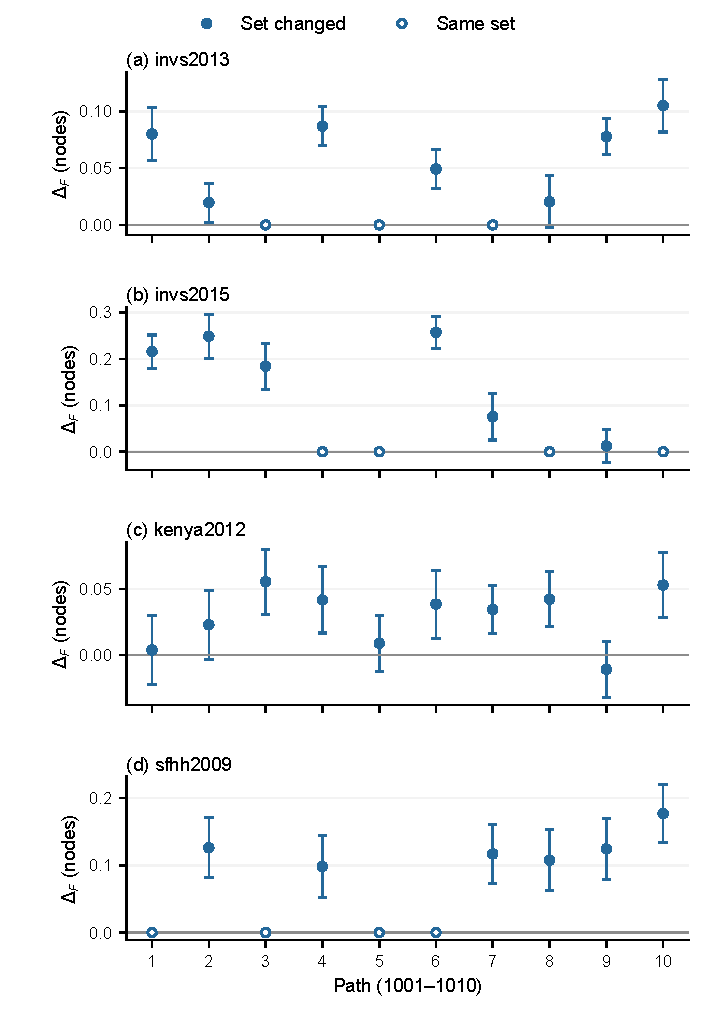
\includegraphics[width=\linewidth]{HistoryEdgeTransitions.pdf}
\caption{Contact-graph study fixed-edge full-reference changes from $W=320$ to 1280.
Each point is one computational replicate's paired high-minus-low spread difference;
filled points indicate a changed final set. Bars are unadjusted pointwise
$\Delta_F\pm1.96\,\mathrm{SE}_{\rm MC}$ intervals from 10,000 saved paired worlds,
conditional on the selected sets. They do not represent replicate or network
uncertainty. Panel-specific scales are used. All 40 replicates are retained, including
negative and zero differences.}\label{fig:hist-edge-transitions}
\end{figure}
\FloatBarrier

\subsection{Larger seed budget and fixed synthetic instances}
Table~\ref{tab:hist-secondary} reports the secondary controls separately. At
$k=20$, a nominal 4k pool contains all 75 kenya2012 vertices. Its exact agreement
is therefore a full-candidate consistency check, not evidence of useful pruning.
The invs2013 pool retains 80/91 vertices (87.91\%), and invs2015 retains 80/212
(37.74\%); these coverage levels differ substantially from the SNAP 20-node
pools. No sfhh2009 configuration with $k=20$ was executed in this extension.

The synthetic controls use one BA instance with attachment parameter 3 and one
SBM instance with four 500-vertex blocks, within-block probability .012 and
between-block probability .0005; graph-generation seed is 20261015. Both have
2,000 vertices and reciprocal arcs. Their weights derive from topology rather
than observed contact events, so Weighted-4k is not independent observed-event
evidence. At $W=320$, all three displayed rankings reproduce all five BA
trajectories. On the fixed SBM instance, Degree-4k and PageRank-4k reproduce 1/5
and 0/5, with mean spread differences of $+0.04052$ and $+0.03756$ nodes. These
are finite-reference comparisons on two fixed graphs; five replicates per graph do
not constitute five independently generated networks.
\begin{longtable}{llrrrrr}
\caption{Secondary contact-graph study controls: $k=20$ for the three contact graphs and $k=5$ for the two fixed synthetic instances; $p=.01$, $h=3$, step coupling. D, P and W denote Degree-4k, PageRank-4k and Weighted-4k. $\Delta$ is restricted minus full spread (nodes); SD is across replicates; loss is the mean pathwise incremental loss (\%), negative when restricted spread exceeds full-reference spread. Match counts refer to the entire ordered sequence. Coverage is the fraction of eligible vertices (\%). Synthetic W denotes topology-derived weights, not observed event frequency.}\label{tab:hist-secondary}\\
\toprule
$W$ & Rank & $\overline\Delta$ & SD & Loss & Match & Cov. \\
\midrule
\endfirsthead
\multicolumn{7}{l}{\tablename~\thetable{} (continued)}\\
\toprule
$W$ & Rank & $\overline\Delta$ & SD & Loss & Match & Cov. \\
\midrule
\endhead
\bottomrule
\endfoot
\multicolumn{7}{l}{\textit{invs2013}}\\*
320 & D & +0.0000 & 0.0000 & +0.00 & 10/10 & 87.91\\*
320 & P & +0.0000 & 0.0000 & +0.00 & 10/10 & 87.91\\*
320 & W & -0.0006 & 0.0019 & +0.02 & 9/10 & 87.91\\*
1280 & D & +0.0000 & 0.0000 & +0.00 & 10/10 & 87.91\\*
1280 & P & +0.0000 & 0.0000 & +0.00 & 10/10 & 87.91\\*
1280 & W & +0.0000 & 0.0000 & +0.00 & 10/10 & 87.91\\
\multicolumn{7}{l}{\textit{invs2015}}\\*
320 & D & +0.0268 & 0.0462 & -0.22 & 5/10 & 37.74\\*
320 & P & +0.0265 & 0.0464 & -0.22 & 6/10 & 37.74\\*
320 & W & -0.0066 & 0.1290 & +0.05 & 0/10 & 37.74\\*
1280 & D & +0.0078 & 0.0247 & -0.06 & 9/10 & 37.74\\*
1280 & P & +0.0000 & 0.0000 & +0.00 & 10/10 & 37.74\\*
1280 & W & -0.1162 & 0.0565 & +0.92 & 0/10 & 37.74\\
\multicolumn{7}{l}{\textit{kenya2012}}\\*
320 & D & +0.0000 & 0.0000 & +0.00 & 10/10 & 100.00\\*
320 & P & +0.0000 & 0.0000 & +0.00 & 10/10 & 100.00\\*
320 & W & +0.0000 & 0.0000 & +0.00 & 10/10 & 100.00\\*
1280 & D & +0.0000 & 0.0000 & +0.00 & 10/10 & 100.00\\*
1280 & P & +0.0000 & 0.0000 & +0.00 & 10/10 & 100.00\\*
1280 & W & +0.0000 & 0.0000 & +0.00 & 10/10 & 100.00\\
\pagebreak[4]
\multicolumn{7}{l}{\textit{synthetic\_ba2000}}\\*
80 & D & +0.0000 & 0.0000 & +0.00 & 5/5 & 1.00\\*
80 & P & +0.0000 & 0.0000 & +0.00 & 5/5 & 1.00\\*
80 & W & +0.0000 & 0.0000 & +0.00 & 5/5 & 1.00\\*
320 & D & +0.0000 & 0.0000 & +0.00 & 5/5 & 1.00\\*
320 & P & +0.0000 & 0.0000 & +0.00 & 5/5 & 1.00\\*
320 & W & +0.0000 & 0.0000 & +0.00 & 5/5 & 1.00\\
\multicolumn{7}{l}{\textit{synthetic\_sbm2000}}\\*
80 & D & +0.1326 & 0.0542 & -21.80 & 0/5 & 1.00\\*
80 & P & +0.1307 & 0.0537 & -21.46 & 0/5 & 1.00\\*
80 & W & +0.1326 & 0.0542 & -21.80 & 0/5 & 1.00\\*
320 & D & +0.0405 & 0.0386 & -5.71 & 1/5 & 1.00\\*
320 & P & +0.0376 & 0.0241 & -5.23 & 0/5 & 1.00\\*
320 & W & +0.0405 & 0.0386 & -5.71 & 1/5 & 1.00\\
\end{longtable}


\subsection{Traceability and scope}
The contact-graph study tables and figures are generated from saved results and metadata
by \texttt{src/integrate\_historical.py}. All-method CSVs retain method metrics,
within-replicate random means, group summaries, candidate coverage and reference
transitions; figure-source CSVs contain every displayed value.
\texttt{REPRODUCE.md} records the aggregation commands and checks.

Contact-graph study controls describe sensitivity on the tested contact networks;
parameter coverage on the SNAP networks remains narrow. Their descriptive
summaries neither add independent SNAP replicates nor change the post-hoc
identity of the PageRank control. The cost comparisons retain the exhaustive
full-candidate reference used in the experiments.
